\documentclass[10pt,leqno]{amsart}
\usepackage{graphicx}
\usepackage{indentfirst,csquotes}
\usepackage{booktabs}
\usepackage{amsmath,amssymb,amsthm}
\usepackage{xcolor,hyperref,paralist,titlesec,fancyhdr,etoolbox}
\usepackage[numbers,sort&compress]{natbib}

\topmargin= .5cm
\textheight= 20cm
\textwidth= 32cc
\baselineskip=16pt
\evensidemargin= .9cm
\oddsidemargin= .9cm

\hypersetup{colorlinks=true, linkcolor=black, filecolor=black, urlcolor=blue, citecolor=blue}

\titleformat{\section}[display]{\normalfont\huge\bfseries\centering}{\centering\chaptertitlename\thechapter}{10pt}{\Large}
\titlespacing*{\section}{0pt}{0ex}{0ex}

\newtheorem{theorem}{Theorem}[]
\newtheorem{definition}[theorem]{Definition}
\newtheorem{example}[theorem]{Example}
\newtheorem{lemma}[theorem]{Lemma}
\newtheorem{proposition}[theorem]{Proposition}
\newtheorem{corollary}[theorem]{Corollary}
\newtheorem{conjecture}[theorem]{Conjecture}

\begin{document}

\title{Eureka-from-CLIP: Replacing CLIP's Text Encoder with Lightweight BERT Adaptation for Zero-Shot Image-Text Retrieval}

\author{Siyuan Zhang$^{*\dagger}$\quad Yadi Cheng$^{\dagger}$\\[4pt]
  \small Zhejiang University of Technology\\
  \small\texttt{\{zhangsiyuan,chengyadi\}@zjut.edu.cn}}


\maketitle

\let\thefootnote\relax
\footnotetext{$^{*}$Corresponding author.}
\footnotetext{$^{\dagger}$Equal contribution.}

\begin{abstract}
We present Eureka-from-CLIP, a framework that replaces CLIP's original text encoder with a lightweight BERT-based encoder for text-to-image retrieval under tight resource constraints. Trained on a single GeForce RTX 4060 Laptop GPU (8 GB VRAM) with only 1.35M trainable LoRA \citep{hu2022lora} parameters, our best BERT-uncased model achieves 60.48\% text-to-image R@1 on Flickr30k \citep{plummer2015flickr30k}, outperforming the native CLIP ViT-B/32 encoder (57.90\%) while using a tiny fraction of its trainable parameters. The same model attains 74.60\% image-to-text R@1, closely matching CLIP's 76.90\%. To compensate for the small batch size mandated by limited GPU memory, we employ a contrastive queue that supplies abundant negatives; crucially, we mask stale text embeddings in the queue to prevent gradient contamination while retaining the full image queue for the text-to-image direction. We further extend BERT to multilingual settings: a multilingual BERT trained solely on English captions achieves 57.08\% / 27.22\% text-to-image R@1 on English and zero-shot Chinese Flickr30k respectively, using captions translated by HY-MT1.5~\citep{hymt152025tencent}. This work provides a practical recipe for replacing CLIP's text encoder with arbitrary BERT variants under limited compute.
\end{abstract}

\bigskip

\section{Introduction}

Vision-language models have become a cornerstone of modern multimodal AI. CLIP \citep{radford2021clip}, trained on 400 million image-text pairs with a contrastive objective, demonstrates remarkable zero-shot transfer capabilities across diverse visual recognition tasks. CLIP consists of a vision encoder and a text encoder whose embeddings are aligned in a shared representation space. While CLIP's text encoder is a 63M-parameter Transformer, many applications require custom text encoders --- for multilingual support, domain-specific vocabulary, or computational efficiency.

However, replacing CLIP's text encoder is non-trivial because the new encoder must align with CLIP's frozen visual embedding space. Naively fine-tuning a text encoder with a contrastive objective often leads to suboptimal retrieval performance.

Our objective is text-to-image (t2i) retrieval: given a natural language query, retrieve the most relevant image or video scene. In this paradigm, the query encoder (text) is the component we directly control and adapt, while the visual encoder only needs to provide a fixed, high-quality feature space. We therefore freeze the CLIP vision encoder and train only the text encoder to align with the fixed visual space, enabling efficient training under limited computational resources.

Under limited GPU memory, we adopt LoRA~\citep{hu2022lora} for parameter-efficient adaptation and employ a queue-based contrastive objective~\citep{he2020moco} to compensate for the small batch size.

To address the staleness issue introduced by training only the text encoder, we retain an image-side queue composed of embeddings from the frozen CLIP vision encoder while masking stale text embeddings. This asymmetric queue design supplies abundant image negatives for t2i learning without introducing stale text representations.

In this work, we propose Eureka-from-CLIP, a framework that replaces CLIP's original text encoder with a BERT-based encoder \citep{devlin2019bert} through contrastive distillation. Our key contributions are:

\begin{enumerate}
    \item We introduce a text-staleness-aware asymmetric queue mechanism that prevents stale text embeddings from contaminating the gradient while retaining the fresh image queue to supply abundant negatives for text-to-image learning under small-batch constraints.
    \item We demonstrate that under tight resource constraints (single 8\,GB GPU, 1.35M trainable parameters, COCO-only training), a BERT-uncased encoder with LoRA adaptation can match and even surpass CLIP's native text encoder on Flickr30k zero-shot retrieval.
    \item We demonstrate zero-shot cross-lingual transfer: a multilingual BERT model trained exclusively on English captions achieves non-trivial Chinese Flickr30k retrieval performance, using machine-translated captions via HY-MT1.5~\citep{hymt152025tencent}.
\end{enumerate}

Our best BERT-uncased model achieves 60.48\% t2i R@1 on Flickr30k, surpassing CLIP's native text encoder while using only 1.35M trainable parameters. We further demonstrate non-trivial zero-shot Chinese retrieval using multilingual BERT trained solely on English captions.

\section{Related Work}

\subsection{Contrastive Vision-Language Pre-training}

CLIP \citep{radford2021clip} introduced a large-scale contrastive learning paradigm that trains vision and language encoders jointly on 400M image-text pairs. The InfoNCE loss \citep{oord2018representation} is used to maximize the similarity of positive pairs while pushing apart negative pairs. Subsequent works have improved upon CLIP in various directions: OpenCLIP provides open-source reproductions, and SigLIP \citep{zhai2023sigmoid} adopts a sigmoid loss for decoupling batch size from performance.

\subsection{Replacing CLIP's Text Encoder}

AltCLIP \citep{chen2022altclip} replaces CLIP's text encoder with XLM-R \citep{conneau2020xlmr} for multilingual capabilities, using a two-stage training process of teacher distillation followed by contrastive learning. Chinese CLIP \citep{yang2022chinese} builds a Chinese-specific vision-language model from scratch with a two-stage training strategy. Our work differs from these approaches in that we focus on a lightweight adaptation of BERT \citep{devlin2019bert} to match CLIP's existing embedding space, requiring only a fraction of the training data and compute.

\subsection{Parameter-Efficient Fine-Tuning}

LoRA \citep{hu2022lora} proposes low-rank decomposition matrices as lightweight adaptations inserted into pre-trained Transformer layers, dramatically reducing the number of trainable parameters. We apply LoRA to BERT's self-attention layers, training only 1.35M parameters (1.2\% of BERT's total parameters) while freezing all original weights.

\subsection{Queue-based Contrastive Learning}

MoCo \citep{he2020moco} introduces a queue-based dictionary for contrastive learning, decoupling dictionary size from batch size. This is especially valuable in resource-constrained settings where the batch size is limited by GPU memory. However, when the encoder being trained produces embeddings that evolve over time, queue entries become stale. Our work directly addresses this staleness issue: we completely mask the text queue for the image-to-text direction, ensuring that only in-batch negatives are used, while retaining the image queue for text-to-image learning (where images come from a frozen CLIP encoder and thus have zero staleness).

\section{Method}

\subsection{Overview}

Our framework replaces CLIP's text encoder with a BERT encoder followed by a lightweight projection head. Because our target task is text-to-image retrieval and CLIP's vision encoder already provides a high-quality frozen feature space, we freeze the vision encoder entirely and train only the text encoder to align with this fixed visual space. This design choice brings three practical benefits: (1) the vision encoder runs only once offline, precomputing embeddings for the entire training set; (2) training reduces to a text-only forward pass, dramatically lowering GPU memory; and (3) the frozen image encoder eliminates the staleness problem for the image side of the contrastive queue. During training, we sample image-text pairs from COCO captions, load the precomputed CLIP image embeddings, and train the BERT encoder to produce text embeddings that align with them in the shared space.

\begin{figure}[h]
\centering
\includegraphics[width=\textwidth]{figures/figure1.png}
\caption{Training pipeline of Eureka-from-CLIP. Frozen CLIP vision encoder precomputes image embeddings (never stale). Trainable BERT text encoder with LoRA produces text embeddings. The image queue supplies abundant negatives for t2i learning, while the stale text queue is masked out.}
\label{fig:pipeline}
\end{figure}

\subsection{Model Architecture}

The model consists of three components:

\textbf{Frozen CLIP Vision Encoder.} We use OpenAI's ViT-B/32 as the frozen vision encoder. All images are encoded once offline, producing 512-dimensional L2-normalized embeddings.

\textbf{BERT Text Encoder.} We use BERT-base (uncased) as the text encoder backbone. For each input caption, BERT's [CLS] token representation is extracted from the final layer.

\textbf{Projection Head.} A linear projection maps the 768-dimensional BERT [CLS] embedding to the 512-dimensional shared space, followed by L2 normalization.

\textbf{LoRA Adapters.} We insert LoRA \citep{hu2022lora} adapters with rank $r=8$ and $\alpha=16$ into BERT's query, key, value, and output projection layers. The original BERT weights remain frozen; only the LoRA parameters and projection head are trainable. This results in only 1.35M trainable parameters out of 110.8M total.

\subsection{Loss Design}

We employ a weighted asymmetric InfoNCE loss \citep{oord2018representation} formulated as:

\begin{equation}
\mathcal{L} = (1 - \alpha) \cdot \text{CE}(\mathbf{S}_{i2t} \cdot \tau, \mathbf{y}) + \alpha \cdot \text{CE}(\mathbf{S}_{t2i} \cdot \tau, \mathbf{y}),
\label{eq:asymmetric_loss}
\end{equation}

where $\mathbf{S}_{i2t} = \mathbf{I} \mathbf{T}^{\top}$ is the image-to-text similarity matrix, $\mathbf{S}_{t2i} = \mathbf{T} \mathbf{I}^{\top}$ is the text-to-image similarity matrix, $\tau = \exp(\gamma)$ is a learnable temperature parameter initialized to $1/0.07$, $\mathbf{y}$ is the set of diagonal labels (positive pairs), $\text{CE}$ denotes cross-entropy, and $\alpha$ is the t2i weight.

We set $\alpha = 0.75$, giving 3$\times$ more weight to the text-to-image direction. This design choice is motivated by real-world usage: in text-to-image retrieval, the user provides a text query and the system retrieves relevant images or scenes, making text-to-image recall the more important metric.

\subsection{Queue Design with Text Staleness Masking}

Contrastive learning benefits from a large number of negative samples. Following MoCo \citep{he2020moco}, we maintain a FIFO queue of past (image, text) embedding pairs. However, a key challenge arises: the text encoder is being trained, so text embeddings in the queue were produced by earlier, less capable versions of the model. These ``stale'' text embeddings, if used as negatives for the image-to-text direction, can provide misleading gradient signals.

Our core insight is that this staleness is direction-dependent, and the asymmetry aligns perfectly with our task objective:

\begin{itemize}
    \item \textbf{Image-to-text (i2t):} The text queue is stale (text encoder evolves). We completely mask the text queue for this direction, using only in-batch negatives. This effectively means $\mathbf{S}_{i2t}$ in Eq.~\ref{eq:asymmetric_loss} is computed as $\mathbf{I}_{\text{batch}} \mathbf{T}_{\text{batch}}^{\top}$ without queue entries. Since t2i is our primary concern, sacrificing i2t queue negatives is an acceptable trade-off.
    \item \textbf{Text-to-image (t2i):} The image queue is \emph{not} stale because image embeddings come from a frozen CLIP encoder. We therefore retain the full image queue for this direction, computing $\mathbf{S}_{t2i} = \mathbf{T}_{\text{batch}} [\mathbf{I}_{\text{batch}}; \mathbf{I}_{\text{queue}}]^{\top}$. The fresh image queue provides a large and consistent set of negatives that directly boosts t2i performance.
\end{itemize}

This asymmetric queue design is illustrated in Table~\ref{tab:queue}. Importantly, the choice of which encoder to train and which queue side to keep is not arbitrary. If we had chosen to train the vision encoder while freezing the text encoder, the image embeddings would become stale and the text queue would remain fresh; the queue would then boost i2t instead of t2i --- the opposite of what we need. Our configuration (training text encoder, retaining the image queue) therefore creates a natural alignment between the training objective and the architectural design: the frozen CLIP guarantees a fresh image queue, and the fresh image queue guarantees strong t2i learning. By masking stale text embeddings, we further avoid damaging the i2t gradient, which is doubly beneficial since t2i already receives higher weight in the loss ($\alpha = 0.75$).

\begin{table}[h]
\centering
\caption{Asymmetric queue design for text-staleness-aware contrastive learning.}
\label{tab:queue}
\begin{tabular}{c|c}
\hline
\textbf{i2t direction} & \textbf{t2i direction} \\
In-batch negatives only & In-batch + queue negatives \\
\hline
$\mathbf{I}_{\text{batch}} \mathbf{T}_{\text{batch}}^{\top}$ & $\mathbf{T}_{\text{batch}} [\mathbf{I}_{\text{batch}}; \mathbf{I}_{\text{queue}}]^{\top}$ \\
No queue (avoid stale texts) & Image queue (no staleness) \\
\hline
\end{tabular}
\end{table}

We additionally apply false-negative masking: queue entries sharing the same image ID as a batch item are masked out (set to $-\infty$) in the similarity matrix, preventing them from being treated as negatives.

\subsection{Training Details}

We train on COCO train2017 captions (113k images, 567k captions) using a single GeForce RTX 4060 Laptop GPU with 8 GB VRAM. The training configuration uses:
\begin{itemize}
    \item Batch size: 128 (maximum that fits in 8 GB VRAM with BERT-base + LoRA)
    \item Optimizer: AdamW with learning rate $3\times 10^{-4}$, weight decay 0.01
    \item Scheduler: Linear warmup (34,536 steps) followed by cosine decay to zero
    \item Epochs: 30
    \item Mixed precision (AMP) for computational efficiency
    \item Queue size: 49,152 (compensates for small batch by providing abundant negatives)
    \item LoRA rank: 8, alpha: 16, dropout: 0.1
\end{itemize}
The queue is updated after loss computation to prevent current-batch items from acting as their own negatives. Precomputed CLIP image embeddings avoid redundant vision forward passes, further reducing GPU memory usage. The entire training run completes in approximately 12 hours.

\section{Experiments}

\subsection{Evaluation Setup}

We evaluate on Flickr30k \citep{plummer2015flickr30k}, which contains 31,783 images, each with 5 human-annotated captions. Following the standard zero-shot retrieval protocol, we use the 1,000-image test set and report Recall@K (R@K) for both image-to-text (i2t) and text-to-image (t2i) directions.

For the CLIP baseline, we use the official OpenAI ViT-B/32 model to encode both images and captions. For the image side, this is the same frozen encoder used during BERT training. For the text side, we use CLIP's native Transformer text encoder.

For the Chinese Flickr30k evaluation, we use the Flickr30k images paired with Chinese translations. The Chinese captions were produced by translating the original English captions using HY-MT1.5~\citep{hymt152025tencent}, a multilingual machine translation model developed by Tencent Hunyuan. We evaluate a multilingual BERT (bert-base-multilingual-cased) model trained with identical hyperparameters on the same COCO English captions. This tests zero-shot cross-lingual generalization: the model has never seen Chinese text during training.

\subsection{Main Results}

Table~\ref{tab:results} presents the main experimental results.

\begin{table}[h]
\centering
\caption{Recall@K on Flickr30k test set (1K images). ``Ours'' refers to models trained with our framework using COCO captions only.}
\label{tab:results}
\begin{tabular}{lcccccc}
\toprule
Method & t2i R@1 & t2i R@5 & t2i R@10 & i2t R@1 & i2t R@5 & i2t R@10 \\
\midrule
CLIP ViT-B/32 (zero-shot) & 57.90 & 82.98 & 89.06 & 76.90 & 94.30 & 97.80 \\
BERT-uncased (EN, Ours)   & 60.48 & 84.96 & 91.00 & 74.60 & 92.90 & 96.60 \\
\midrule
Multilingual BERT (EN, Ours) & 57.08 & 82.38 & 89.62 & 69.00 & 91.40 & 95.30 \\
Multilingual BERT (ZH, Ours) & 27.22 & 56.22 & 66.94 & 39.20 & 69.00 & 78.90 \\
\bottomrule
\end{tabular}
\end{table}

Our BERT-uncased model achieves highly competitive performance:
\begin{itemize}
    \item \textbf{Text-to-image:} R@1 of 60.48\%, \emph{outperforming} CLIP's 57.90\% by 2.6 points, despite training on a single RTX 4060 GPU with only COCO captions. This validates the effectiveness of our text-staleness-aware queue mechanism and retrieval-oriented training strategy.
    \item \textbf{Image-to-text:} R@1 of 74.60\%, which is within 2.3 points of CLIP's 76.90\%, with only 1.35M trainable parameters.
\end{itemize}

The multilingual BERT, trained with identical hyperparameters on the same English COCO data:
\begin{itemize}
    \item Achieves 57.08\% t2i R@1 on English Flickr30k, a reasonable degradation from BERT-uncased (60.48\%) due to the multilingual tokenizer's reduced efficiency for English text.
    \item Attains 27.22\% t2i R@1 on Chinese Flickr30k in a zero-shot cross-lingual setting --- substantially above the random baseline of 0.1\%, demonstrating meaningful cross-lingual transfer.
\end{itemize}

\subsection{Analysis: Impact of Asymmetric Loss and Queue Design}

\begin{table}[h]
\centering
\begin{tabular}{lcc}
\toprule
Configuration & t2i R@1 & i2t R@1 \\
\midrule
Ours (full) & 60.48 & 74.60 \\
w/o mask (stale text queue allowed) & 44.32 & 53.80 \\
w/o queue & 55.06 & 72.10 \\
\bottomrule
\end{tabular}
\caption{Ablation of queue components in our framework.}
\label{tab:ablation}
\end{table}

\begin{table}[h]
\centering
\begin{tabular}{lcc}
\toprule
$\alpha$ (t2i weight) & t2i R@1 & i2t R@1 \\
\midrule
0.25 & 59.28 & 76.10 \\
0.50 & 60.26 & 75.90 \\
0.75 & 60.48 & 74.60 \\
\bottomrule
\end{tabular}
\caption{Effect of the asymmetric loss weight $\alpha$ on retrieval performance.}
\label{tab:alpha}
\end{table}

Table~\ref{tab:ablation} summarizes ablation experiments. Removing the text-staleness mask (``w/o mask'') severely degrades both directions, as stale text embeddings contaminate the gradient. This setting is notably worse than ``w/o queue'', indicating that an unmasked queue actively harms learning more than having no queue at all. Without the queue (``w/o queue''), the lack of abundant negatives primarily hurts t2i.

Table~\ref{tab:alpha} examines the effect of the loss weight $\alpha$. Increasing $\alpha$ from 0.25 to 0.75 yields only a modest +1.20 t2i R@1 gain (from 59.28 to 60.48), with a corresponding shift from i2t toward t2i. The $\alpha{=}0.50$ configuration achieves 60.26 t2i R@1, only 0.22 points below the full $\alpha{=}0.75$ setting, indicating that the asymmetric loss weight contributes relatively little compared to the queue design.

\subsection{Ablation: Parameter Distribution (LoRA vs.\ MLP Projection)}

To isolate whether the performance gains of LoRA stem from additional trainable capacity or from its layer-wise distribution within BERT, we replace all LoRA adapters with a three-layer MLP projection head ($768 \to 704 \to 704 \to 512$) that has a comparable number of trainable parameters (${\sim}$1.40M versus ${\sim}$1.35M in the LoRA configuration). The MLP is inserted after BERT's [CLS] pooling, replacing both the original linear projection head and the LoRA adapters. All other hyperparameters remain identical.

Table~\ref{tab:ablation_mlp} reports the results. The MLP projection achieves only 39.92\% t2i R@1 and 51.3\% i2t R@1, substantially below the LoRA configuration (60.48\% / 74.60\%) and even below the ``w/o queue'' ablation (55.06\% / 72.10\%). This 20+ point drop in t2i R@1 demonstrates that the architectural placement of trainable parameters is far more important than their raw count. LoRA's effectiveness lies in its ability to adapt BERT's internal representations across all 12 Transformer layers, whereas the MLP concentrates all trainable capacity in a single post-hoc projection that cannot compensate for the frozen BERT backbone's misalignment with CLIP's embedding space.

Interestingly, the MLP configuration also exhibits a plateau in validation loss after the early epochs (val\_loss reaches a minimum of 2.44 at epoch 5 and then gradually increases), suggesting that the post-hoc projection quickly exhausts its representational capacity. In contrast, the LoRA configuration continues to improve throughout the 30-epoch training schedule.

\begin{table}[h]
\centering
\caption{Ablation: LoRA vs.\ MLP projection with comparable parameter counts. Both models are trained on COCO and evaluated zero-shot on Flickr30k.}
\label{tab:ablation_mlp}
\begin{tabular}{lcccccc}
\toprule
Method & t2i R@1 & t2i R@5 & t2i R@10 & i2t R@1 & i2t R@5 & i2t R@10 \\
\midrule
LoRA (Ours) & 60.48 & 84.96 & 91.00 & 74.60 & 92.90 & 96.60 \\
MLP projection & 39.92 & 68.88 & 78.68 & 51.30 & 81.00 & 89.20 \\
\bottomrule
\end{tabular}
\end{table}

\section{Discussion}

\subsection{Queue Asymmetry Dominates Retrieval Optimization}

The ablation results in Tables~\ref{tab:ablation} and~\ref{tab:alpha} reveal a clear hierarchy among our design choices. Removing the queue entirely degrades t2i R@1 by 5.42 points (from 60.48 to 55.06), while reducing the t2i weight $\alpha$ from 0.75 to 0.50 shifts only 0.22 points (from 60.26 to 60.48, Table~\ref{tab:alpha}). The performance gain from the queue is considerably larger than that obtained by explicit loss reweighting.

The text-staleness mask is even more critical: allowing stale text embeddings into the queue (``w/o mask'') collapses t2i R@1 to 44.32, a drop of 16.16 points. An unmasked queue is worse than no queue at all, indicating that stale gradients from outdated text embeddings actively harm learning rather than merely providing diminishing returns.

These results demonstrate that the largest performance gain in our framework originates from the asymmetric queue mechanism rather than from explicit loss reweighting.

\subsection{Why Is Loss Reweighting Less Important Than Expected?}

The relatively modest impact of $\alpha$ can be understood by examining the loss dynamics during training. The image queue supplies a large number of additional negatives exclusively for the text-to-image direction, making the t2i task inherently harder than i2t within each batch. This asymmetry originates from the large image queue, which introduces tens of thousands of additional image negatives for the t2i branch. Consequently, the raw t2i loss is consistently larger than the corresponding i2t loss during training. Figure~\ref{fig:loss_ratio} plots the unweighted loss ratio $L_{t2i}/L_{i2t}$ over the full training trajectory (with $\alpha{=}0.75$). Notably, the ratio rises from approximately 3.3$\times$ in the first epoch to over 13.5$\times$ by convergence, with a mean of $11.86\times$ across all epochs. This trend is counterintuitive: despite assigning a larger optimization weight ($\alpha{=}0.75$) to the t2i branch, the raw t2i loss not only remains higher but continues to diverge from i2t throughout training. If loss weighting were the dominant factor, one would expect the raw t2i loss to approach the i2t loss as training progresses. Instead, the growing ratio indicates that the queue-induced difficulty overwhelms the compensation from explicit reweighting, confirming that queue asymmetry --- rather than loss weighting --- is the primary driver of t2i optimization bias.

This observation explains why the $\alpha{=}0.50$ configuration (Table~\ref{tab:alpha}) achieves 60.26 t2i R@1, only 0.22 points below $\alpha{=}0.75$. The queue, by asymmetrically supplying more negatives to t2i, serves as an implicit regularizer that reduces the need for explicit loss weighting.

\begin{figure}[h]
\centering
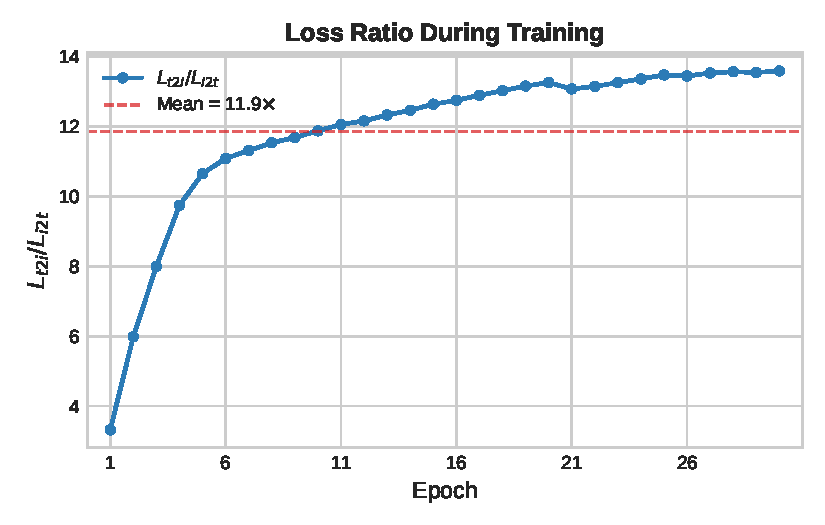
\includegraphics[width=0.72\textwidth]{figures/loss_ratio.pdf}
\caption{
\label{fig:loss_ratio}
Ratio of raw (unweighted) text-to-image loss to image-to-text loss $L_{t2i}/L_{i2t}$ during training with $\alpha{=}0.75$.
Despite the explicit optimization bias favoring t2i, the ratio increases from approximately 3.3$\times$ in the first epoch to over 13.5$\times$ by convergence, with a mean of $11.86\times$ (dashed line).
This growing gap demonstrates that the queue-induced asymmetry dominates the effect of loss reweighting.
}
\end{figure}

\subsection{Resource Constraints Naturally Lead to the Asymmetric Design}

The asymmetric queue is not an arbitrary design choice. Rather, it emerges naturally from our resource-constrained training setup: freezing the CLIP vision encoder keeps image embeddings perpetually fresh, while the evolving text encoder renders queued text embeddings stale. Under this setup, retaining only the image queue becomes the most natural solution.

\section{Limitations}

We acknowledge several limitations in this work. First, our models are trained exclusively on COCO train2017 captions (113k images, 567k captions), a single dataset with limited domain diversity. While this allows us to demonstrate the effectiveness of our approach under tight compute constraints, training on a more diverse corpus (e.g., CC-3M~\citep{sharma2018conceptual} or YFCC100M~\citep{thomee2016yfcc100m}) would likely improve generalization.

Second, evaluation is conducted solely on Flickr30k, a benchmark that is similar in domain and scale to COCO (both contain natural scene photographs with human-annotated captions). We do not evaluate on out-of-domain or challenging retrieval benchmarks such as MS-COCO itself as a test set, or on cross-domain generalization tasks. The relatively small 1K test set also means that R@K metrics may have higher variance than would be expected on larger benchmarks.

Third, the zero-shot cross-lingual evaluation is limited to Chinese on a single dataset, using machine-translated rather than human-annotated captions. The translation quality of HY-MT1.5~\citep{hymt152025tencent} may introduce noise that underestimates the true cross-lingual transfer capability.

Fourth, the ablation experiments in Table~\ref{tab:ablation} report single-run results without confidence intervals. Due to compute constraints, each configuration was evaluated once rather than with multiple random seeds, so the observed differences should be interpreted with caution.

\section{Future Work}

Several directions are worth exploring. The most immediate extension is to video retrieval, where a text query must retrieve relevant video clips. This requires aggregating per-frame CLIP embeddings into a video-level representation. Simple approaches such as mean pooling over a frame pool can serve as a baseline, while more sophisticated temporal encoding --- for example, a lightweight Transformer or temporal convolution over the frame embedding sequence --- could capture motion and event structure. Our preliminary experiments indicate that training such a temporal module against frozen CLIP frame embeddings, using the same contrastive framework, is a natural extension of the approach presented here.

Additional future directions include: evaluating on a broader set of benchmarks spanning diverse domains (e.g., MS-COCO test set, Visual Genome, and cross-domain retrieval); exploring larger BERT variants or alternative text encoders with more aggressive parameter efficiency; and extending the framework to support retrieval in additional modalities.

\section{Conclusion}

We presented Eureka-from-CLIP, a framework for replacing CLIP's text encoder with a lightweight BERT adapter under tight resource constraints. Trained on a single RTX 4060 Laptop GPU (8 GB VRAM) with only 1.35M trainable LoRA parameters, our BERT-uncased model outperforms CLIP's native text encoder on text-to-image Flickr30k retrieval (60.48\% vs.~57.90\% t2i R@1) while remaining competitive on image-to-text. Through a text-staleness-aware asymmetric queue design and parameter-efficient fine-tuning, we achieve this with a fraction of the compute required by prior work. Furthermore, we demonstrate that multilingual BERT exhibits non-trivial zero-shot cross-lingual transfer to Chinese without any Chinese training data.

Our approach provides a practical, generalizable recipe for substituting CLIP's text encoder with arbitrary BERT variants, enabling multilingual and domain-specific applications without expensive retraining from scratch. More broadly, our results suggest that adapting the text encoder alone, when coupled with an appropriate queue design, can be a practical alternative to full vision-language retraining under limited computational budgets.

\section*{Acknowledgments}

The authors thank Jie Lei for guidance and helpful discussions throughout this project. This work was completed as a course project for Python Application Development Foundation at Zhejiang University of Technology.

\bigskip

\bibliographystyle{plainnat}
\begin{thebibliography}{99}

\bibitem[Radford et al.(2021)Radford, Kim, Hallacy, Ramesh, Goh, Agarwal, Sastry, Askell, Mishkin, Clark, Krueger, and Sutskever]{radford2021clip}
A.~Radford, J.~W.~Kim, C.~Hallacy, A.~Ramesh, G.~Goh, S.~Agarwal, G.~Sastry, A.~Askell, P.~Mishkin, J.~Clark, G.~Krueger, and I.~Sutskever.
\newblock Learning transferable visual models from natural language supervision.
\newblock In \textit{ICML}, 2021.

\bibitem[Devlin et al.(2019)Devlin, Chang, Lee, and Toutanova]{devlin2019bert}
J.~Devlin, M.-W.~Chang, K.~Lee, and K.~Toutanova.
\newblock BERT: Pre-training of deep bidirectional transformers for language understanding.
\newblock In \textit{NAACL-HLT}, 2019.

\bibitem[He et al.(2020)He, Fan, Wu, Xie, and Girshick]{he2020moco}
K.~He, H.~Fan, Y.~Wu, S.~Xie, and R.~Girshick.
\newblock Momentum contrast for unsupervised visual representation learning.
\newblock In \textit{CVPR}, 2020.

\bibitem[Hu et al.(2022)Hu, Shen, Wallis, Allen-Zhu, Li, Wang, Wang, and Chen]{hu2022lora}
E.~J.~Hu, Y.~Shen, P.~Wallis, Z.~Allen-Zhu, Y.~Li, S.~Wang, L.~Wang, and W.~Chen.
\newblock LoRA: Low-rank adaptation of large language models.
\newblock In \textit{ICLR}, 2022.

\bibitem[Chen et al.(2022)Chen, Liu, Zhang, Ye, Yang, and Wu]{chen2022altclip}
Z.~Chen, G.~Liu, B.-W.~Zhang, F.~Ye, Q.~Yang, and L.~Y.~Wu.
\newblock AltCLIP: Altering the language encoder in CLIP for extended language capabilities.
\newblock \textit{arXiv preprint arXiv:2211.06679}, 2022.

\bibitem[Yang et al.(2022)Yang, Pan, Lin, Men, Zhang, Zhou, and Zhou]{yang2022chinese}
A.~Yang, J.~Pan, J.~Lin, R.~Men, Y.~Zhang, J.~Zhou, and C.~Zhou.
\newblock Chinese CLIP: Contrastive vision-language pretraining in Chinese.
\newblock \textit{arXiv preprint arXiv:2211.01335}, 2022.

\bibitem[van den Oord et al.(2018)van den Oord, Li, and Vinyals]{oord2018representation}
A.~van den Oord, Y.~Li, and O.~Vinyals.
\newblock Representation learning with contrastive predictive coding.
\newblock \textit{arXiv preprint arXiv:1807.03748}, 2018.

\bibitem[Plummer et al.(2015)Plummer, Wang, Cervantes, Caicedo, Hockenmaier, and Lazebnik]{plummer2015flickr30k}
B.~A.~Plummer, L.~Wang, C.~M.~Cervantes, J.~C.~Caicedo, J.~Hockenmaier, and S.~Lazebnik.
\newblock Flickr30k entities: Collecting region-to-phrase correspondences for richer image-to-sentence models.
\newblock In \textit{ICCV}, 2015.

\bibitem[Lin et al.(2014)Lin, Maire, Belongie, Hays, Perona, Ramanan, Dollár, and Zitnick]{lin2014coco}
T.-Y.~Lin, M.~Maire, S.~Belongie, J.~Hays, P.~Perona, D.~Ramanan, P.~Dollár, and C.~L.~Zitnick.
\newblock Microsoft COCO: Common objects in context.
\newblock In \textit{ECCV}, 2014.

\bibitem[Conneau et al.(2020)Conneau, Khandelwal, Goyal, Chaudhary, Wenzek, Guzmán, Grave, Ott, Zettlemoyer, and Stoyanov]{conneau2020xlmr}
A.~Conneau, K.~Khandelwal, N.~Goyal, V.~Chaudhary, G.~Wenzek, F.~Guzmán, E.~Grave, M.~Ott, L.~Zettlemoyer, and V.~Stoyanov.
\newblock Unsupervised cross-lingual representation learning at scale.
\newblock In \textit{ACL}, 2020.

\bibitem[Zhai et al.(2023)Zhai, Mustafa, Kolesnikov, and Beyer]{zhai2023sigmoid}
X.~Zhai, B.~Mustafa, A.~Kolesnikov, and L.~Beyer.
\newblock Sigmoid loss for language image pre-training.
\newblock In \textit{ICCV}, 2023.

\bibitem[Sharma et al.(2018)Sharma, Ding, and
  Soricut]{sharma2018conceptual}
P.~Sharma, N.~Ding, and R.~Soricut.
\newblock Conceptual captions: A cleaned, hypernymed, image alt-text dataset for
  automatic image captioning.
\newblock In \textit{ACL}, 2018.

\bibitem[Thomee et al.(2016)Thomee, Shamma, Friedland, Elizalde, Ni, Poland,
  Borth, and Li]{thomee2016yfcc100m}
B.~Thomee, D.~A.~Shamma, G.~Friedland, B.~Elizalde, K.~Ni, D.~Poland,
  D.~Borth, and L.-J.~Li.
\newblock YFCC100M: The new data in multimedia research.
\newblock \textit{Communications of the ACM}, 59(2):64--73, 2016.

\bibitem[Tencent Hunyuan Team(2025)]{hymt152025tencent}
Tencent Hunyuan Team.
\newblock HY-MT1.5 technical report.
\newblock \textit{arXiv preprint arXiv:2512.24092}, 2025.

\end{thebibliography}

\section{Hyperparameter Selection}

We evaluate $\alpha \in \{0.25, 0.50, 0.75\}$. Although $\alpha{=}0.50$ already achieves comparable performance, $\alpha{=}0.75$ yields the highest t2i R@1 and is therefore adopted in the final model. Table~\ref{tab:hyperparams} summarizes the key hyperparameters used in our framework. All experiments use LoRA rank $r=8$ trained on COCO captions with seed 42.

\begin{table}[h]
\centering
\caption{Key hyperparameters. CLIP ViT-B/32 (OpenAI) baseline: t2i R@1~57.90\%, i2t R@1~76.90\%.}
\label{tab:hyperparams}
\begin{tabular}{lcc}
\toprule
Hyperparameter & Value & Description \\
\midrule
Batch size & 128 & Max for 8 GB VRAM \\
Learning rate & $3\times10^{-4}$ & AdamW, cosine decay \\
Weight decay & 0.01 & \\
Warmup steps & 34,536 & Linear warmup \\
Epochs & 30 & \\
\midrule
LoRA rank $r$ & 8 & \\
LoRA $\alpha$ & 16 & \\
LoRA dropout & 0.1 & \\
LoRA targets & Q, K, V, O & BERT linear layers \\
\midrule
Queue size & 49,152 & FIFO contrastive queue \\
t2i weight $\alpha$ & 0.75 & Eq.~\ref{eq:asymmetric_loss} \\
Temperature $\tau$ init & $1/0.07$ & Learnable $\tau=\exp(\gamma)$ \\
\midrule
AMP & true & Mixed precision \\
\bottomrule
\end{tabular}
\end{table}

\end{document}
